% Options for packages loaded elsewhere
\PassOptionsToPackage{unicode}{hyperref}
\PassOptionsToPackage{hyphens}{url}
\PassOptionsToPackage{dvipsnames,svgnames,x11names}{xcolor}
%
\documentclass[
  letterpaper,
  DIV=11,
  numbers=noendperiod]{scrartcl}

\usepackage{amsmath,amssymb}
\usepackage{iftex}
\ifPDFTeX
  \usepackage[T1]{fontenc}
  \usepackage[utf8]{inputenc}
  \usepackage{textcomp} % provide euro and other symbols
\else % if luatex or xetex
  \usepackage{unicode-math}
  \defaultfontfeatures{Scale=MatchLowercase}
  \defaultfontfeatures[\rmfamily]{Ligatures=TeX,Scale=1}
\fi
\usepackage{lmodern}
\ifPDFTeX\else  
    % xetex/luatex font selection
\fi
% Use upquote if available, for straight quotes in verbatim environments
\IfFileExists{upquote.sty}{\usepackage{upquote}}{}
\IfFileExists{microtype.sty}{% use microtype if available
  \usepackage[]{microtype}
  \UseMicrotypeSet[protrusion]{basicmath} % disable protrusion for tt fonts
}{}
\makeatletter
\@ifundefined{KOMAClassName}{% if non-KOMA class
  \IfFileExists{parskip.sty}{%
    \usepackage{parskip}
  }{% else
    \setlength{\parindent}{0pt}
    \setlength{\parskip}{6pt plus 2pt minus 1pt}}
}{% if KOMA class
  \KOMAoptions{parskip=half}}
\makeatother
\usepackage{xcolor}
\setlength{\emergencystretch}{3em} % prevent overfull lines
\setcounter{secnumdepth}{-\maxdimen} % remove section numbering
% Make \paragraph and \subparagraph free-standing
\makeatletter
\ifx\paragraph\undefined\else
  \let\oldparagraph\paragraph
  \renewcommand{\paragraph}{
    \@ifstar
      \xxxParagraphStar
      \xxxParagraphNoStar
  }
  \newcommand{\xxxParagraphStar}[1]{\oldparagraph*{#1}\mbox{}}
  \newcommand{\xxxParagraphNoStar}[1]{\oldparagraph{#1}\mbox{}}
\fi
\ifx\subparagraph\undefined\else
  \let\oldsubparagraph\subparagraph
  \renewcommand{\subparagraph}{
    \@ifstar
      \xxxSubParagraphStar
      \xxxSubParagraphNoStar
  }
  \newcommand{\xxxSubParagraphStar}[1]{\oldsubparagraph*{#1}\mbox{}}
  \newcommand{\xxxSubParagraphNoStar}[1]{\oldsubparagraph{#1}\mbox{}}
\fi
\makeatother


\providecommand{\tightlist}{%
  \setlength{\itemsep}{0pt}\setlength{\parskip}{0pt}}\usepackage{longtable,booktabs,array}
\usepackage{calc} % for calculating minipage widths
% Correct order of tables after \paragraph or \subparagraph
\usepackage{etoolbox}
\makeatletter
\patchcmd\longtable{\par}{\if@noskipsec\mbox{}\fi\par}{}{}
\makeatother
% Allow footnotes in longtable head/foot
\IfFileExists{footnotehyper.sty}{\usepackage{footnotehyper}}{\usepackage{footnote}}
\makesavenoteenv{longtable}
\usepackage{graphicx}
\makeatletter
\newsavebox\pandoc@box
\newcommand*\pandocbounded[1]{% scales image to fit in text height/width
  \sbox\pandoc@box{#1}%
  \Gscale@div\@tempa{\textheight}{\dimexpr\ht\pandoc@box+\dp\pandoc@box\relax}%
  \Gscale@div\@tempb{\linewidth}{\wd\pandoc@box}%
  \ifdim\@tempb\p@<\@tempa\p@\let\@tempa\@tempb\fi% select the smaller of both
  \ifdim\@tempa\p@<\p@\scalebox{\@tempa}{\usebox\pandoc@box}%
  \else\usebox{\pandoc@box}%
  \fi%
}
% Set default figure placement to htbp
\def\fps@figure{htbp}
\makeatother
% definitions for citeproc citations
\NewDocumentCommand\citeproctext{}{}
\NewDocumentCommand\citeproc{mm}{%
  \begingroup\def\citeproctext{#2}\cite{#1}\endgroup}
\makeatletter
 % allow citations to break across lines
 \let\@cite@ofmt\@firstofone
 % avoid brackets around text for \cite:
 \def\@biblabel#1{}
 \def\@cite#1#2{{#1\if@tempswa , #2\fi}}
\makeatother
\newlength{\cslhangindent}
\setlength{\cslhangindent}{1.5em}
\newlength{\csllabelwidth}
\setlength{\csllabelwidth}{3em}
\newenvironment{CSLReferences}[2] % #1 hanging-indent, #2 entry-spacing
 {\begin{list}{}{%
  \setlength{\itemindent}{0pt}
  \setlength{\leftmargin}{0pt}
  \setlength{\parsep}{0pt}
  % turn on hanging indent if param 1 is 1
  \ifodd #1
   \setlength{\leftmargin}{\cslhangindent}
   \setlength{\itemindent}{-1\cslhangindent}
  \fi
  % set entry spacing
  \setlength{\itemsep}{#2\baselineskip}}}
 {\end{list}}
\usepackage{calc}
\newcommand{\CSLBlock}[1]{\hfill\break\parbox[t]{\linewidth}{\strut\ignorespaces#1\strut}}
\newcommand{\CSLLeftMargin}[1]{\parbox[t]{\csllabelwidth}{\strut#1\strut}}
\newcommand{\CSLRightInline}[1]{\parbox[t]{\linewidth - \csllabelwidth}{\strut#1\strut}}
\newcommand{\CSLIndent}[1]{\hspace{\cslhangindent}#1}

\KOMAoption{captions}{tableheading}
\makeatletter
\@ifpackageloaded{caption}{}{\usepackage{caption}}
\AtBeginDocument{%
\ifdefined\contentsname
  \renewcommand*\contentsname{Table of contents}
\else
  \newcommand\contentsname{Table of contents}
\fi
\ifdefined\listfigurename
  \renewcommand*\listfigurename{List of Figures}
\else
  \newcommand\listfigurename{List of Figures}
\fi
\ifdefined\listtablename
  \renewcommand*\listtablename{List of Tables}
\else
  \newcommand\listtablename{List of Tables}
\fi
\ifdefined\figurename
  \renewcommand*\figurename{Figure}
\else
  \newcommand\figurename{Figure}
\fi
\ifdefined\tablename
  \renewcommand*\tablename{Table}
\else
  \newcommand\tablename{Table}
\fi
}
\@ifpackageloaded{float}{}{\usepackage{float}}
\floatstyle{ruled}
\@ifundefined{c@chapter}{\newfloat{codelisting}{h}{lop}}{\newfloat{codelisting}{h}{lop}[chapter]}
\floatname{codelisting}{Listing}
\newcommand*\listoflistings{\listof{codelisting}{List of Listings}}
\makeatother
\makeatletter
\makeatother
\makeatletter
\@ifpackageloaded{caption}{}{\usepackage{caption}}
\@ifpackageloaded{subcaption}{}{\usepackage{subcaption}}
\makeatother

\usepackage{bookmark}

\IfFileExists{xurl.sty}{\usepackage{xurl}}{} % add URL line breaks if available
\urlstyle{same} % disable monospaced font for URLs
\hypersetup{
  pdftitle={Safe Drinking Water for California Water Systems},
  pdfauthor={Susan Peck},
  colorlinks=true,
  linkcolor={blue},
  filecolor={Maroon},
  citecolor={Blue},
  urlcolor={Blue},
  pdfcreator={LaTeX via pandoc}}


\title{Safe Drinking Water for California Water Systems\thanks{Project
repository available at:
https://github.com/susanpeck/MATH261A-project-1-Linear-Regression}}
\usepackage{etoolbox}
\makeatletter
\providecommand{\subtitle}[1]{% add subtitle to \maketitle
  \apptocmd{\@title}{\par {\large #1 \par}}{}{}
}
\makeatother
\subtitle{At Risk Small and Disadvantaged Communities}
\author{Susan Peck}
\date{September 24, 2025}

\begin{document}
\maketitle


\section{Abstract}\label{sec-abstract}

This will be a great abstract summarizing everything succinctly and also
making sure that people want to read the rest of my paper. It will be
intriguing and informative. I understand that not having an abstract in
my draft means that you can not give me constructive and timely feedback
on this part of my paper.

\section{Introduction}\label{sec-introduction}

California drinking water is safe for 98\% (California State Water
Resources Control Board 2024) of the population and meets state drinking
water standards that are more strict than federal regulations. This
still leaves about 400 failing water systems serving 870,000 people, 600
water systems serving 1.6 million people that are at risk of failure,
and more than 400 others serving another 1.6 million that are
potentially at risk of failing. (California State Water Resources
Control Board 2025) Smaller communities and populations that are
economically disadvantaged may be more at risk of having water with
higher levels of contaminants, or they may not have the resources to
address and fix problems with the water system.

In 2016 the California State Water Resource Board adopted a Human Right
to Water Resolution that includes a statement that ``every human being
has the right to safe, clean, affordable, and accessible water adequate
for human consumption, cooking and sanitary purposes.'' The goals of
Human Right to Water are to provide safe drinking water, accessible
drinking water, affordable drinking water, and/or maintaining a
sustainable and resilient water system. In 2019 California established
the Safe and Affordable Funding for Equity and Resilience (SAFER)
Program with the goal of helping struggling water systems and to help
provide affordable safe drinking water. In 2021 SAFER performed a Needs
Assessment to try to determine where and how funds should be used to
have the most impact in improving failing or at risk water systems and
provided recommendations.

The California State Water Board conducted the risk assessment with 19
indicators across four categories. The categories were Water Quality,
Accessibility, Affordability, and Technical, Managerial, and Financial
(TMF) Capacity. Each year the Needs Assessment was updated and the data
published with risk assessment scores for each category. This paper will
focus on 2024 data and the scores from each of the categories from
communities with fewer than 3300 service connections.

Funding has been provided to try and address inequities in small water
systems and fix problems in a sustainable way. This paper will
investigate to see if there are correlations between economic status of
the population a small water system serves and indicator scores.

This paper will detail the data obtained from the Drinking Water Needs
Assessment and relevant variables, describe the general simple linear
regression model used to analyze potential correlations, and show the
results of the linear regression and residual analysis.

\section{Data}\label{sec-data}

This paper uses data from the 2024 Drinking Water Needs Assessment
report (California State Water Resources Control Board 2024) through the
SAFER program and definitions from the original 2021 Drinking Water
Needs Assessment report (California State Water Resources Control Board
2021). The reports were prepared by the California State Water Resources
Control Board within the California Environmental Protection Agency
(CalEPA), in partnership with the UCLA Luskin Center for Innovation
(UCLA).

The report calculated a risk assessment value for each water system. The
Risk Assessment Result is based off of a score for each of 19 risk
indicators (see figure below). A standardized score is a value between 0
and 1. Weight values between 1 and 3 were applied to the individual risk
indicators. This resulted in a score value for each subcategory. A total
weighted risk value was calculated using the four subcategories scores.
The result was used to indicate if the water system was At-Risk,
Not-At-Risk, or Potentially-At-Risk. Some systems were not evaluated and
have a Not Assessed value.

\begin{center}
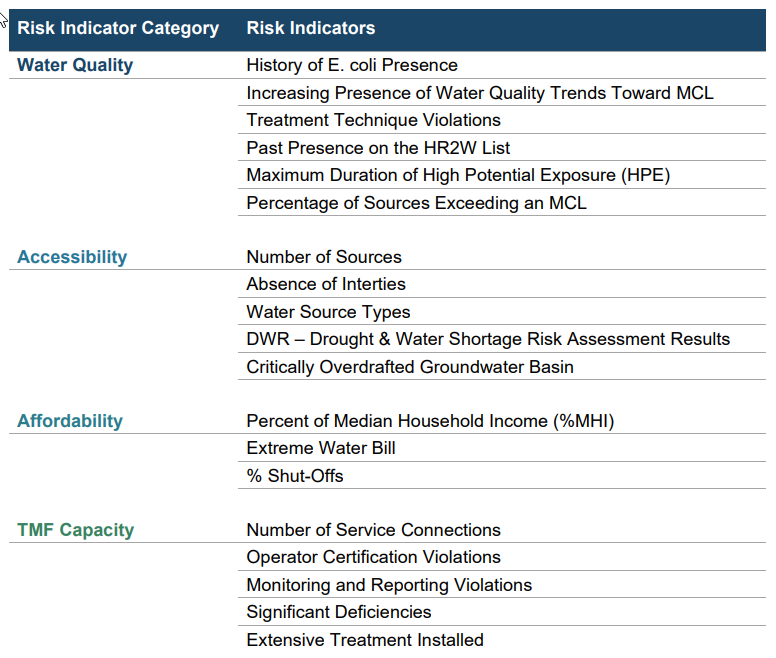
\includegraphics[width=5.64583in,height=\textheight,keepaspectratio]{Risk_Indicators_2021.png}
\end{center}

All ``At Risk'' systems exceed a `threshold of concern' (see
Section~\ref{sec-thresholds} for specific values) for at least four risk
indicators.

This paper looks at the individual subcategory scores from the Risk
Assessment, a California Environmental Screening Score, population, and
Median Household Income (MHI), and investigates the possible
relationships between those variables. The subcategories are Water
Quality, Affordability, Accessibility, and TMF Capacity. (See longer
definitions from the Needs Assessment report
Section~\ref{sec-definitions})

The CalEnviroScreen (\emph{CalEnviroScreen} 2025) is a score created by
the State of California Office of Environmental Health Hazard Assessment
(OEHHA) that uses environmental, health, and socioeconomic information
to produce scores for every census tract in the state. A higher score is
an area that has a higher pollution burden than a lower score. Below is
a scatterplot of the CalEnvironScreen score compared to MHI for that
water system. Only smaller water systems with fewer than 3300 service
connections are included. Each data point is colored to show if the
water system is at risk of failing to provide clean drinking water.

\begin{figure}

\centering{

\pandocbounded{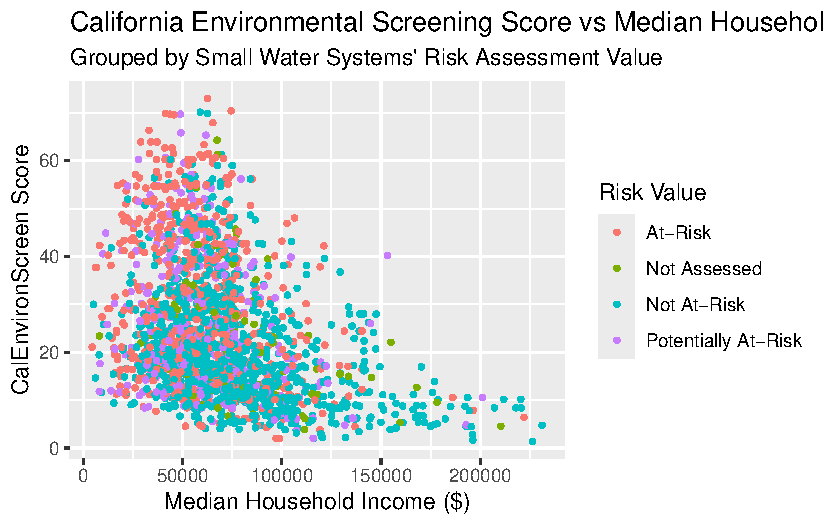
\includegraphics[keepaspectratio]{SusanPeckMath261AProject1Paper_files/figure-pdf/fig-calenviron-mhi-1.pdf}}

}

\caption{\label{fig-calenviron-mhi}Scatter plot of calenvironscreen
versus MHI grouped by risk assessment values}

\end{figure}%

The Median Household Income (MHI) uses the annual income value for all
the people in a single household. The MHI for this data set is the
median household annual income for the population in each water system.
The median household income is a typical value that is used as a general
economic measure and as a way to compare populations. On an individual
level, MHI can be used to determine if you qualify for certain aid. In
this data set MHI is one way to compare different populations served by
different water systems.

The Needs Assessment spent time trying to figure out a threshold for
what would make water unaffordable to the residents of that water
system. Affordability in this data set is based on three measured
values: the percent of the MHI, a comparison to the state average water
bill, and the number of shut-offs of water. Section~\ref{sec-thresholds}

Accessibility is a combination of five indicators that include how many
sources a water system has, if the system is reliant on connetions to
other systems, and what types of sources (groundwater, snow, rivers,
etc.) This score also includes information about droughts and
overdrafted water basins.

TMF Capacity risk indicators measure a system's technical, managerial
and financial (TMF) capacity to actually maintain a water system long
term.

\section{Methods}\label{sec-methods}

This paper looks at the results of a simple linear regression model
shown below.

\[Y_i = \beta_0 +\beta_1 X_i + \varepsilon_i\]

\(Y_i\) represents the response variable. In this paper the first linear
regression analysis the response variable is the CalEnviroScreen Score.

\(X_i\) represents the predictor variable. In this paper the first
linear regression analysis the predictor variable is MHI.

\(\beta_0\) is the y-intercept of the model. For the first linear
regression analysis this would be the expected mean value of the
CalEnviroScreen score for water system population with a median
household income of \$0. A household could have an income of \$0, but it
is unlikely to be a median household income for a population, so this
particular intercept doesn't have a direct interpretation.

\(\beta_1\) is the slope of the model. The slope represents how much the
response variable changes for a unit change in the predictor variable.
In the first regression model the slope would represent how much we
would expect the mean CalEnviroScreen Score to change based on a one
dollar change for the MHI.

\(\varepsilon_i\) are the error terms.

This model assumes a linear relationship between Y and X. If the actual
relationship between Y and X is not a linear one, then the model could
be a bad fit for the data, to the extreme of not being useful at all, or
possibly just have some bias and predictive values are off.

The model also assumes that the error terms are independent, have a
constant variance for all levels of the predictor variable X, the mean
of the error terms is zero, and the error terms are normally
distributed. If these assumptions are not true then the values and
confidence intervals can be misleading. For this data set the sample
size is large enough that the normality assumption is less important.

The analysis was done using R programming \{R Core Team (2025)\} and
built in function, lm, to fit the linear model and provide calculated
estimate values for the slope and intercept of the model. The summary
function of the lm model also shows a p-value for each of the estimates
and a \(R^2\) value.

\section{Results}\label{sec-results}

After a couple years of funding and some improvements to small water
systems in California, are there correlations between risk indicator
scores? To begin this analysis we looked at a scatterplot of the
CalEnviroScreen Score and MHI Figure~\ref{fig-calenviron-mhi} shown in
the Data Section Section~\ref{sec-data} of this paper. The larger the
CalEnviroScreen Score, the more pollution a population is subject to.
General pollution may or may not directly impact water quality. The
scatterplot below indicates lower MHI seems to have more At-Risk water
systems. The larger the value of the MHI for the water system, the fewer
water systems that have high CalEnviroScreen score.

\begin{figure}[H]

{\centering \pandocbounded{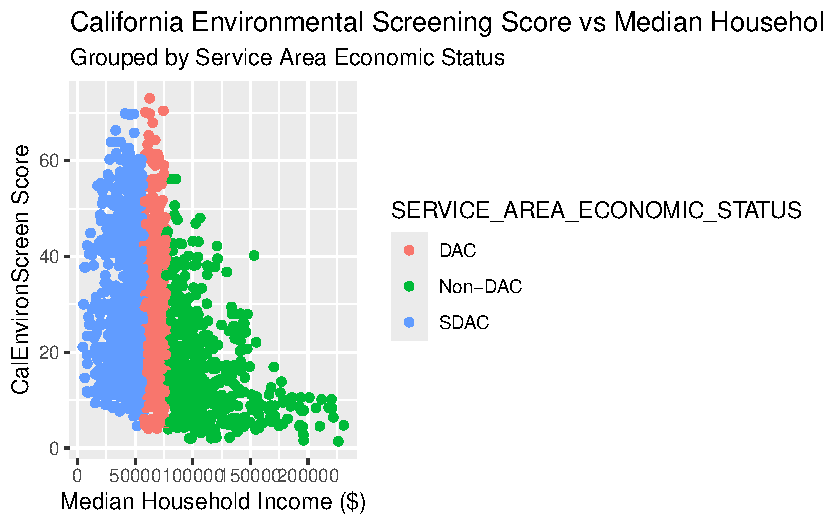
\includegraphics[keepaspectratio]{SusanPeckMath261AProject1Paper_files/figure-pdf/fig_calenviro_mhi_DAC-1.pdf}}

}

\caption{Scatter plot of calenvironscreen versus MHI grouped by service
area economic status}

\end{figure}%

The scatterplot above again graphs CalEnviroScreen Score against MHI,
but this time groups by the economic status of the service area. The
status could be a Disadvantaged Community (DAC), a Severely
Disadvantaged Community (SDAC), or a Non-Disadvantaged Community
(Non-DAC). The classifications of how disadvantaged a community is is a
direct calculation based on MHI, as shown by the vertical sections on
the scatterplot. Both the DAC and SDAC communities have a large range of
CalEnviroScreen Scores. The Non-DAC communities have a smaller range of
values and the values are less in general.

\begin{verbatim}

Call:
lm(formula = CALENVIRO_SCREEN_SCORE ~ MHI, data = water_data_small_systems)

Residuals:
    Min      1Q  Median      3Q     Max 
-22.801  -9.925  -2.530   7.446  48.089 

Coefficients:
              Estimate Std. Error t value Pr(>|t|)    
(Intercept)  3.455e+01  5.540e-01   62.35   <2e-16 ***
MHI         -1.535e-04  7.231e-06  -21.22   <2e-16 ***
---
Signif. codes:  0 '***' 0.001 '**' 0.01 '*' 0.05 '.' 0.1 ' ' 1

Residual standard error: 12.91 on 2772 degrees of freedom
Multiple R-squared:  0.1398,    Adjusted R-squared:  0.1394 
F-statistic: 450.4 on 1 and 2772 DF,  p-value: < 2.2e-16
\end{verbatim}

The SDAC communities CalEnviroScreen Score ranged from 4.551 to 69.86
with and average value of 28.688. The DAC communities CalEnviroScreen
Score ranged from 4.035 to 73.036 with and average value of 24.858.The
Non-DAC communities CalEnviroScreen Score ranged from 1.372 to 56.183
with and average value of 16.389.

The simple linear regression model for this relationship would have a
\(b_0\) value of 34.547 and the \(b_1\) value of
\ensuremath{-2\times 10^{-4}}. As discussed in the Methods Section
Section~\ref{sec-methods}, the intercept \(b_0\) does not have a
relevant meaning for a predictor value of MHI equal to zero. The \(b_1\)
value represents the slope of the linear model and means that for every
dollar increase in the Median Household Income level for a water
system's population, the population has a decreased CalEnviroScreen
Score of about \ensuremath{-2\times 10^{-4}}. The negative slope value
matches the visual impression from the scatterplot that populations with
a higher MHI will have a lower CalEnviroScreen score.

In the model the p-value is small (much smaller than 0.001) for both the
intercept and slope estimates, indicating there may be some significance
to the model. However, the large range of values in the data for each
predictor level, and the smaller \(R^2\) value of
\texttt{r\ lm\_calenviro\_summary\$r.squared} means that the model may
not be the best fit for the data and may not do a good job of explaining
the variance.

The CalEnviroScreen score is the result of several factors that may
contribute to pollution in an area and is not explained purely by the
income level of the local population.

Below is a residual plot from the linear regression model, plotting the
residual against the fitted value. If this plot shows random points
above and below zero with no clear trend then this suggests that the
model could be a good fit for the data. If the residuals show a trend
that is curved or something that is not horizontal at y=0, it could
suggest some of the assumptions in the model are not met.

\begin{figure}[H]

{\centering \pandocbounded{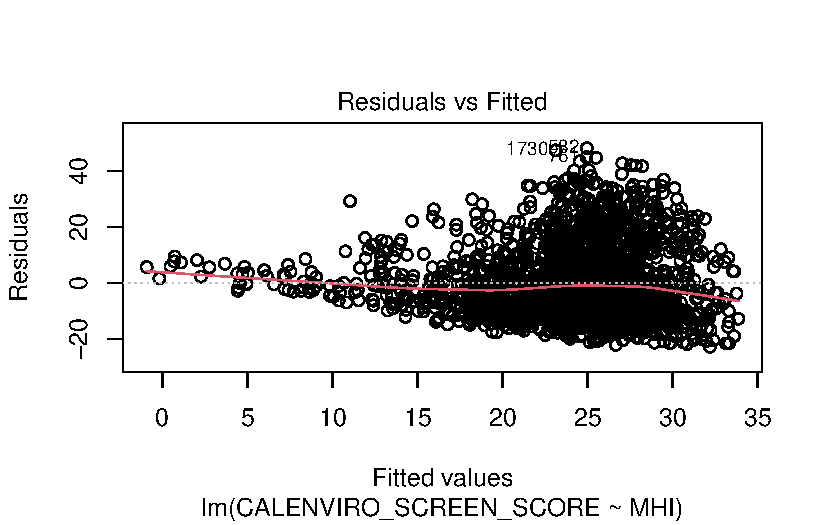
\includegraphics[keepaspectratio]{SusanPeckMath261AProject1Paper_files/figure-pdf/unnamed-chunk-3-1.pdf}}

}

\caption{Residual plot of CalEnvironScreen Score versus MHI}

\end{figure}%

The residual plot above does have a trend. Most of the points on the
left are above the y=0 line, and most of the points on the right are
below the y=0 line. This indicates that the model doesn't explain all of
the variance besides random error.

The residuals also have a wider range on the right of the plot, fanning
out, meaning the assumption of constant variance in the error terms is
not met. The p-test or t-test values may not be reliable.

I would have liked to explore more of the relationships between the
indicator scores and MHI, as well as between the indicator scores to see
if any of them have a linear relationship and what that could mean. I am
not sure how many linear regression analyses would be appropriate in
this project.

\section{Appendix A DEFINITIONS}\label{sec-definitions}

\emph{Affordability Threshold} means the level, point, or value that
delineates if a water system's residential customer charges, designed to
ensure the water systems can provide drinking water that meets State and
Federal standards, are unaffordable. For the purposes of the 2021
Affordability Assessment, the State Water Board employed affordability
thresholds for the following indicators: Percent Median Household
Income; Extreme Water Bill; and Percent Shut-Offs. Learn more about
current and future indicators and affordability thresholds in Appendix
E.

\emph{Affordability Assessment} means the identification of any
community water system that serves a disadvantaged community that must
charge fees that exceed the affordability threshold established by the
State Water Board in order to supply, treat, and distribute potable
water that complies with Federal and state drinking water standards. The
Affordability Assessment evaluates several different affordability
indicators to identify communities that may be experiencing
affordability challenges. (Health \& Saf. Code, § 116769, subd. (2)(B).

\emph{At-Risk public water systems} or \emph{At-Risk PWS} means
community water systems with 3,300 service connections or less and K-12
schools that are at risk of failing to meet one or more key Human Right
to Water goals: (1) providing safe drinking water; (2) accessible
drinking water; (3) affordable drinking water; and/or (4) maintaining a
sustainable water system.

\emph{Median household income} or \emph{MHI} means the household income
that represents the median or middle value for the community. The
methods utilized for calculating median household income are included in
Appendix A and Appendix E. Median household incomes in this document are
estimated values for the purposes of this statewide assessment. Median
household income for determination of funding eligibility is completed
on a system by system basis by the State Water Board's Division of
Financial Assistance.

\emph{Risk indicator} means the quantifiable measurements of key data
points that allow the State Water Board to assess the potential for a
community water system or a transient noncommunity water system that
serves a K-12 school to fail to sustainably provide an adequate supply
of safe drinking water due to water quality, water accessibility,
affordability, institutional, and/or TMF capacity issues.

\emph{Risk threshold} means the levels, points, or values associated
with an individual risk indicator that delineates when a water system is
more at-risk of failing, typically based on regulatory requirements or
industry standards.

\emph{Score} means a standardized numerical value that is scaled between
0 and 1 for risk points across risk indicators. Standardized scores
enable the evaluation and comparison of risk indicators.

\emph{Service connection} means the point of connection between the
customer's piping or constructed conveyance, and the water system's
meter, service pipe, or constructed conveyance, with certain exceptions
set out in the definition in the Health and Safety Code. (See Health \&
Saf. Code, § 116275, subd. (s).)

\emph{Small community water system} means a CWS that serves no more than
3,300 service connections or a yearlong population of no more than
10,000 persons. (Health \& Saf. Code, § 116275, subd. (z).)

\emph{Risk Indicators} means quantifiable measurements of key data
points that allow the State Water Board to assess the probability of a
water system's failure to deliver safe drinking water or other
infrastructure and institutional failures. Risk indicators that measure
water quality, accessibility, affordability, and TMF capacity are
incorporated based on their criticality as it relates to a system's
ability to remain in compliance with safe drinking water standards and
their data availability and quality across the State.

\emph{Risk Indicator Thresholds} are the levels, points, or values
associated with an individual risk indicator that delineates when a
water system is more at-risk of failing.

\emph{Scores \& Weights} are the application of a multiplying value or
weight to each risk indicator and risk category, as certain risk
indicators and categories may be deemed more critical than others and/or
some may be out of the control of the water system. The application of
weights to risk indicators and risk categories allows the State Water
Board multiple ways to assess all risk indicators within each category
together in a combined Risk Assessment score.

\emph{TMF Capacity} risk indicators measure a system's technical,
managerial and financial (TMF) capacity to plan for, achieve, and
maintain long term compliance with drinking water standards, thereby
ensuring the quality and adequacy of the water supply.

\section{Apendix B THRESHOLD VALUES}\label{sec-thresholds}

\begin{center}
\pandocbounded{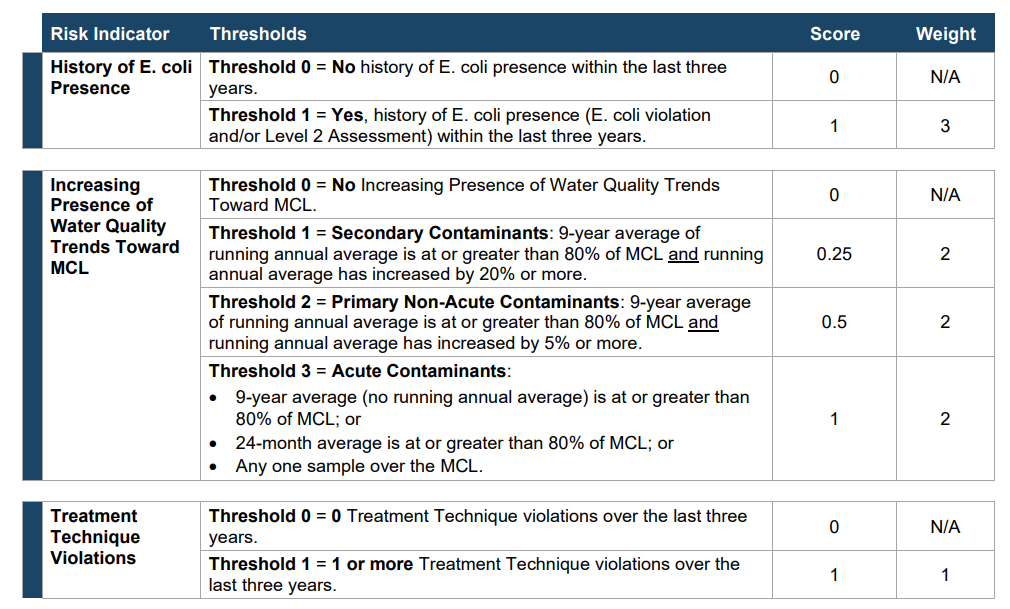
\includegraphics[keepaspectratio]{Thresholds1.png}}
\end{center}

\begin{center}
\pandocbounded{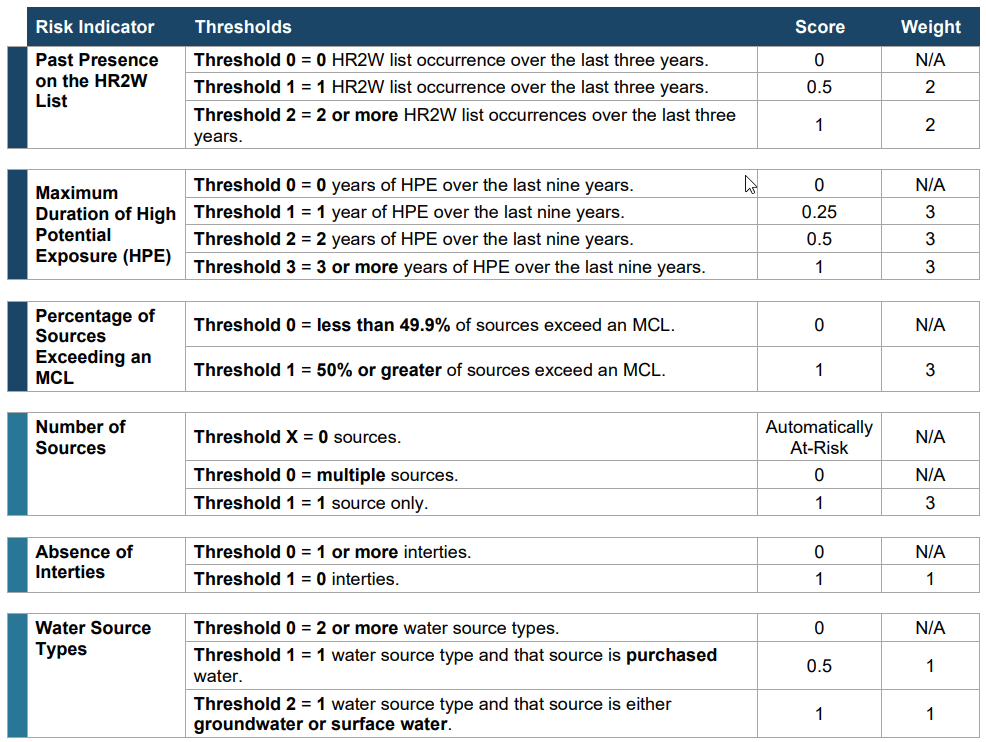
\includegraphics[keepaspectratio]{Thresholds2.png}}
\end{center}

\begin{center}
\pandocbounded{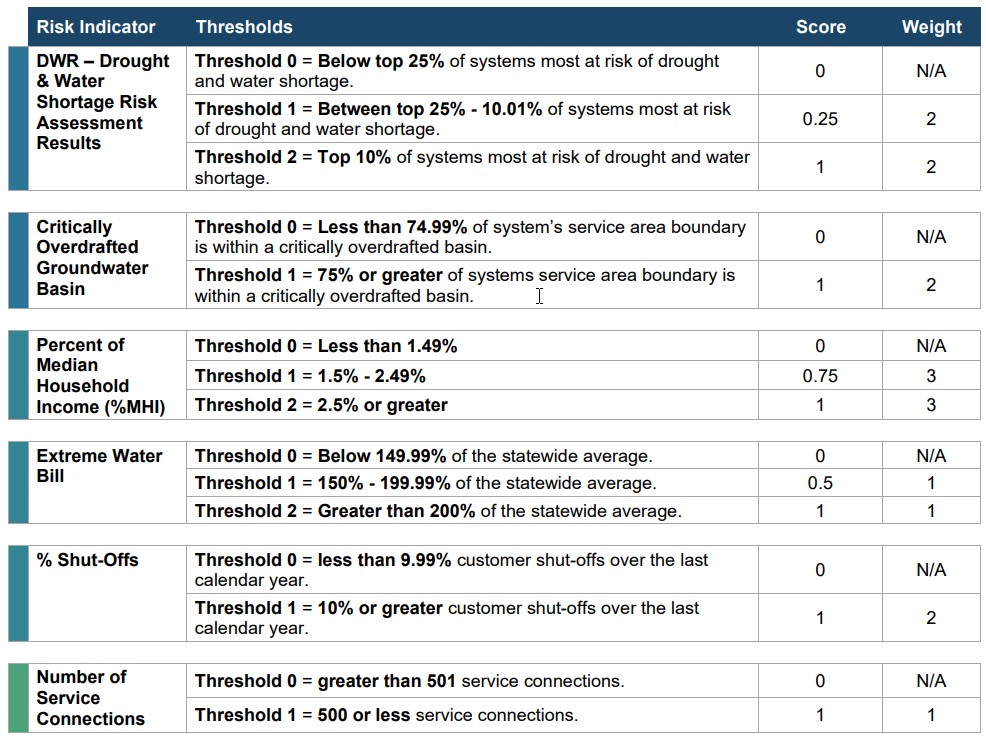
\includegraphics[keepaspectratio]{Thresholds3.png}}
\end{center}

\begin{center}
\pandocbounded{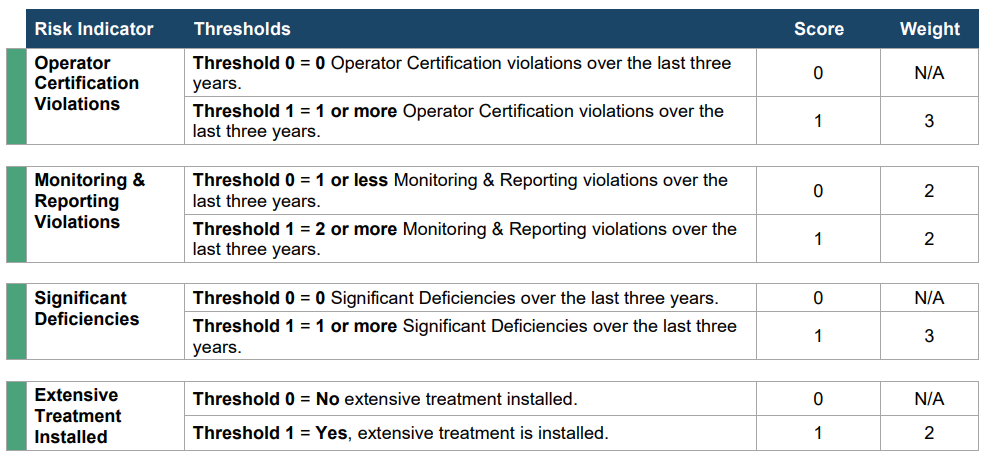
\includegraphics[keepaspectratio]{Thresholds4.png}}
\end{center}

\section*{References}\label{references}
\addcontentsline{toc}{section}{References}

\phantomsection\label{refs}
\begin{CSLReferences}{1}{0}
\bibitem[\citeproctext]{ref-calenviro}
\emph{CalEnviroScreen}. 2025. State of California Office of
Environmental Health Hazard Assessment (OEHHA).
\url{https://oehha.ca.gov/calenviroscreen}.

\bibitem[\citeproctext]{ref-2021needsreport}
California State Water Resources Control Board. 2021. \emph{2021
Drinking Water Needs Assessment Executive Summary}.
\url{https://www.waterboards.ca.gov/drinking_water/certlic/drinkingwater/documents/needs/executive_summary.pdf}.

\bibitem[\citeproctext]{ref-2024needsreport}
---------. 2024. \emph{2024 Drinking Water Needs Assessment Results}.
\url{https://www.waterboards.ca.gov/drinking_water/certlic/drinkingwater/documents/needs/2024/2024-needs-assessment.pdf}.

\bibitem[\citeproctext]{ref-waterfail}
---------. 2025. \emph{2025 SAFER Dashboard}.
\url{https://www.waterboards.ca.gov/drinking_water/certlic/drinkingwater/documents/needs/2024/2024-needs-assessment.pdf}.

\bibitem[\citeproctext]{ref-rcode}
R Core Team. 2025. \emph{R: A Language and Environment for Statistical
Computing}. Vienna, Austria: R Foundation for Statistical Computing.
\url{https://www.R-project.org/}.

\end{CSLReferences}




\end{document}
